\documentclass[../main/main.tex]{subfiles}

% Put everything that shall appear in the introduction
% inside this document environment.
\begin{document}
	The question of how to predict peoples performance on a task has been of great interest in the psychology literature. To be able to make qualified statements about this ability, one has to define it first.
	This can be achieved by the framework of \textit{metacognition} including the frequently used terms \textit{metacognitive sensitivity}, \textit{metacognitive bias} and \textit{metacognitive efficiency}, as presented by \cite{fleming2014measure}, that will be explained during this first section.\\
	\textit{Metacognitive sensitivity} is used to express how good a subject is at differing between his or her own correct and incorrect answers. For example, imagine a classical experiment from \textit{signal detection theory (SDT)} where the subject's task is to rate a stimulus to come from a class A or a distinct class B. Poor metacognitive sensitivity would result in a bad distinction between the possible origins, even though the classes are easy to separate for an average observer. A useful initial approach to quantify \textit{metacognitive sensitivity} is the $2x2$ confidence-accuracy table, labeled \textit{type-2 SDT table} by \cite{fleming2014measure}, that is the equivalent of the usual \textit{type-1 SDT table} [x], shown in the upper part from figure \ref{fig:tables}, applied to the \textit{metacognition} framework. The resulting table is displayed in the lower part of \ref{fig:tables}. Typical SDT measurements of the association between the rows and the columns of the table in the type-1 case are the \textit{$\phi$-correlation}, defined e.g. in \cite{cramer1999mathematical}, and the \textit{Goodman-Kruskall gamma coefficient $G$} from \cite{goodman1963measures}. Imagine a subject reporting a subjective confidence for multiple trials of the former example stored in a vector, e.g $(A, B, B, A)$, and the vector of the actual correct classifications $(A, B, A, B)$. If we encode $A=1$ and $B=0$, the $\phi$-correlation is the \textit{Pearson r-correlation} between both vectors. The advantage of using $G$ instead is the abundance of any distributional assumptions on the data and the possibility to easily extend the measurement to a confidence rating scale (e.g. from 0 to 100), rather than a binary encoding (e.g. 0/1). Nevertheless it is well known that both measurements are affected by bias \cite{fleming2014measure}. \cite{nelson1984comparison} and \cite{masson2009sources} could show that this also holds for the type-2 application of these measurements.
	\begin{figure}[H]
		\centering
		\captionsetup{justification=centering}
		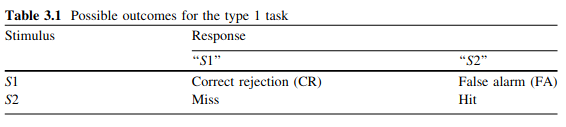
\includegraphics[width=0.7\textwidth]{../assets/type1_sdt_table.png}
		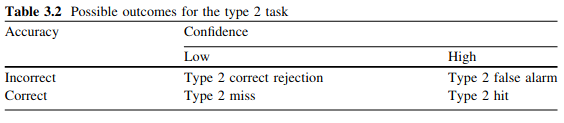
\includegraphics[width=0.7\textwidth]{../assets/type2_sdt_table.png}
		\caption{The type-1 and type-2 2x2 SDT-tables as explained in \cite{fleming2014measure}.} 
		\label{fig:tables}
	\end{figure}
	A standard way to remove the influence of the bias in classic SDT is using $d'$ as in \cite{green1966signal} which will be constant given different biases and also has several approaches to metacognitive sensitivity, e.g. \cite{kunimoto2001confidence} defined type-2 $d'$ as
	\begin{displaymath}
		d' = z(H2) - z(FA2)
	\end{displaymath}
	A visualization of this measurement is shown on the left side of figure \ref{fig:d_dash_and_roc}.
	\begin{figure}[H]
		\centering
		\captionsetup{justification=centering}
		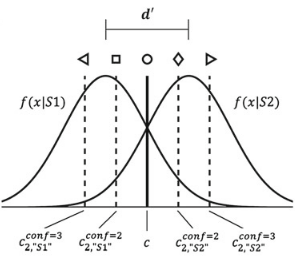
\includegraphics[width=0.5\textwidth]{../assets/d_dash.png}
		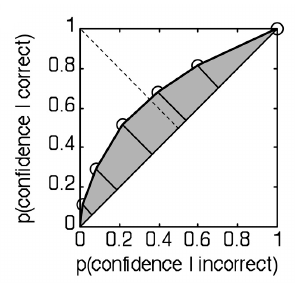
\includegraphics[width=0.45\textwidth]{../assets/type1_roc.png}
		\caption{The left side of this figure shows an example for the d' measurement, calculated as the difference between the (inverse of) the hit rate (HR) and the false alarm rate (FA). The right side displays an example for a type-2 ROC curve, displaying the relationship between FA2 and HR2. The area under the ROC, called \textit{AUROC} gives a measurement of a subject's metacognitive sensitivity.} 
		\label{fig:d_dash_and_roc}
	\end{figure}
	Despite this advantage, $d'$ can not easily applied to the type-2 data, because it includes assumptions of gaussian distributions with equal variance, which is very unlikely to be the case in type-2 data, as shown by \cite{galvin2003type}. Experiments of these \cite{azzopardi2007evaluation} showed that it is indeed affected by changes in the metacognitive bias.\\
	One way to remove this issue is the use of non-parametric analysis, that does not make these assumptions, e.g. the \textit{Receiver operating characteristic (ROC)} analysis [x] in classic SDT. This approach can be applied to type-2 data analogue to \cite{clarke1959two} and an example is given in the right part of figure \ref{fig:d_dash_and_roc}\\
	A further complication for using the above methods to measure metacognitive sensitivity is the fact that all these measures are affected by the task performance \cite{galvin2003type}. This can be addressed by explicitly modeling the connection between a subject's performance and metacognition in a model-based approach. The \textit{meta-$d'$} measure, defined by \cite{maniscalco2012signal}, makes use of the fact that given gaussian variance assumptions at type-1 level, the shapes of the type-2 distributions are known even if they are not themselves gaussian. Therefore the optimal type-2 performance is constrained by one's type-1 performance. E.g. given a particular type-1 variance structure and bias, the form of the type-2 ROC can be completely determined. So, given a subject's actual type-2 performance, one could reconstruct the underlying type-1 sensitivity, labeled meta-$d'$, that is robust to changes in the bias and recovers simulated changes in metacognitive sensitivity, e.g. by altering task difficulties. For a metacognitive ideal observer, meta-$d'$ should be equal to $d'$. To measure this quantity, \cite{fleming2014measure} defined \textit{metacognitive efficiency} as the ratio of meta-$d'/d'$, or by the more stable variants meta-$d'-d'$ or $log$meta-$d'/d'$. However, this measurement is unable to discriminate between different causes of a change in metacognitive efficiency. For example,  trial-to-trial variability in the placement of confidence criteria results in decreasing efficiency as well as additional noise in the evidence used to make the confidence rating. A similar bias-free approach to model metacognitive accuracy is the \textit{Stochastic Detection and Retrieval Model (SDRM)} from \cite{jang2012stochastic} which we do not want to cover here.\\
	A somewhat different approach uses so-called \textit{one-shot} discrepancy measures to quantify metacognition, e.g. in \cite{kruger1999unskilled}. A general confidence rating (Asked before of after the trials) is compared to the actual performance on a variety of tasks, but it should be clear from the above that using a single rating of performance will not result in a good distinction between the bias and sensitivity, nor will it enable to measure the efficiency. In contrast, collecting trial-by-trial measures of performance and metacognitive judgments allows to get a picture of an individuals bias, sensitivity and efficiency.\\
	To get a different view-point on the domain, one could formalize metacognitive confidence as the ability to make good probability judgments directed towards the accuracy of one's own actions.
	
	\subsection{Formalizing metacognition as probability judgments}
	
	In this framework \textit{metacognition} gets a normative interpretation as the accuracy of a probability judgment about one's own performance and one advantage is the possibility to elicit a meaningful measure of the bias. A lot of literature is a available on how to measure this accuracy, but in the following we want to focus on one of them, called the \textit{Brier Score}. To define this score, \cite{fleming2014measure} first defined the \textit{Probability Score (PS)}, analogue to \cite{harvey1997confidence}, as the squared difference between a probability rating $f$ for an event, and it's actual occurrence $c$ (0 or 1 for binary events):
	\begin{displaymath}
			PS = (f - c)^2
	\end{displaymath}
	Based on this, the \textit{Brier Score (BS)} from \cite{brier1950verification} can then be defined as the mean value of the PS averaged across all estimates:
	\begin{displaymath}
			BS = \frac{1}{N}\sum_i(f_i - c_i)^2
	\end{displaymath}
	This score is an equivalent of the $\phi$ or $G$ measurements explained above and can be decomposed, as shown by \cite{murphy1973new}, in the following way:
	\begin{displaymath}
		BS = O + C - R
	\end{displaymath}
	where $O$ is the \textit{Outcome Index}, reflecting the variance of the outcome event $c$:
	\begin{displaymath}
		O = \bar{c}(1-\bar{c})
	\end{displaymath}
	The \textit{Calibration} expresses the goodness of fit between the probability assessments and the corresponding proportion of correct responses. It quantifies the discrepancy between the mean performance level in a category (e.g. $60\%$) and its associated rating (e.g. $80\%$):
	\begin{displaymath}
		C = \frac{1}{N}\sum_{j=1}^{N}N_j(f_j - \bar{c_j})
	\end{displaymath}
	Last, the \textit{Resolution} $R$ encodes the variance of the probability assessments, measuring the extent to which correct and incorrect answers are assigned to different probability categories:
	\begin{displaymath}
		R = \frac{1}{N}\sum_{j=1}^{N}N_j(\bar{c_j} - \bar{c})
	\end{displaymath}
	As mentioned earlier, this framework allows us to extract more meaningful quantities about a subject's metacognitive sensitivity. One such quantity is the calibration of a subject, as shown in figure \ref{fig:calibration}, that directly shows over- or underconfident tendencies of a person.
	\begin{figure}[H]
		\centering
		\captionsetup{justification=centering}
		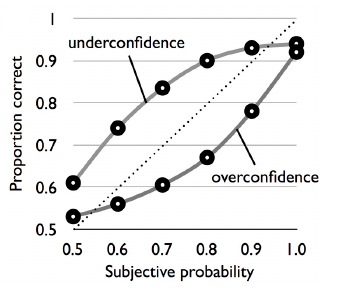
\includegraphics[width=0.55\textwidth]{../assets/calibration_curve.png}
		\caption{TODO: CAPTION} 
		\label{fig:calibration}
	\end{figure}
	For multiple possible outcome classes, the brier score can be calculated as shown by \cite{brier1950verification} by summing over all classes $j$:
	\begin{displaymath}
		BS = \frac{1}{N}\sum_j\sum_i(f_{ij} - c_{ij})^2
	\end{displaymath}
	Note that this formulation does have a range of scores from 0.0 to 2.0, where the analogue values of the one-class formulation are twice as high, e.g. a brier score of 0.5 in the one-class case would correspond to a score of 1.0 in the multi-class formulation.\\
	The next chapter gives explains our methods to actually capture a subjects confidence and calculate a measure of the brier score out of it. We present an experiment that we evaluated on several subjects for different tasks, before we display the results of our measurements in chapter \ref{sec:results} and finally come to a conclusion on our attempt to measure metacognition in chapter \ref{sec:discussion}.
	

\end{document}